\section{Введение и классификация}
\selectlanguage{russian}

Блоковые шифры являются основой современной криптографии. Многие криптографические примитивы -- криптографически стойкие генераторы псевдослучайной последовательности (см. главу~\ref{chapter-crypto-random}), криптографические функции хэширования (см. главу~\ref{chapter-hash-functions}) основаны так или иначе на блоковых шифрах. А использование медленной криптографии с открытым ключом было бы невозможно по практическим соображениям без быстрых блоковых шифров.

Блоковые шифры можно рассматривать как функцию преобразования строки фиксированной длины в строку аналогичной длины\footnote{В случае использования недетерминированных алгоритмов, дающих новый результат при каждом шифровании, длина выхода будет больше. Меньше длина выхода быть не может, так как будет невозможно однозначно восстановить произвольное сообщение.} с использованием некоторого ключа, а также соответствующую ей функцию расшифрования:
\[\begin{array}{l}
	C = E_K\left( M \right), \\
	M'= D_K\left( C \right).
\end{array}\]

Данные функции необходимо дополнить требованиями корректности, производительности и надежности. Во-первых, функция расшифрования должна однозначно восстанавливать произвольное исходное сообщение:

\[ \forall k \in \group{K}, m \in \group{M}: D_k \left( E_k\left( m \right) \right) = m. \]

Во-вторых, функции шифрования и расшифрования должны быстро выполняться легальными пользователями (знающими ключ). В-третьих,  должно быть невозможно найти открытый текст сообщения по шифротексту без знания ключа, кроме как полным перебором всех возможных ключей расшифрования. Также, что менее очевидно, надёжная функция блокового шифра не должна давать возможность найти ключ шифрования (расшифрования) даже если злоумышленнику известны пары открытого текста и шифротекста. Последнее свойство защищает от атак на основе известного открытого текста\index{атака!с известным открытым текстом} и на основе известного шифротекста\index{атака!с известным шифротекстом}, а также активно используется при построении криптографических функций хэширования в конструкции Миагучи---Пренеля\index{Миагучи---Пренеля, конструкция}. То есть:
\begin{itemize}
	\item $C = f \left( M, K \right)$ и $M = f \left( C, K \right)$ должны вычисляться быстро (легальные операции);
	\item $M = f \left( C )$ и $C = f \left( M \right)$ должны вычисляться не быстрее, чем $\left| \group{K} \right|$ операций расшифрования (шифрования), при условии, что злоумышленник может отличить корректное сообщение (см. выводы к разделу~\ref{section_unicity_distance});
	\item $K = f \left( M, C \right)$ должно вычисляться не быстрее, чем $\left| \group{K} \right|$ операций шифрования;
\end{itemize}

Если размер ключа достаточно большой (от 128 бит и выше), то функцию блокового шифрования, удовлетворяющую указанным выше условиям, можно называть надёжной.

Блоковые шифры делят на два больших класса по методу построения.
\begin{itemize}
	\item Шифры, основанные на SP-сетях (сети замены-перестановки), основанные на \textit{обратимых} преобразованиях с открытым текстом. При разработке таких шифров криптограф должен следить за тем, чтобы каждая из производимых операций была и криптографически надёжна, и обратима при знании ключа.
	\item Шифры, в той или иной степени построенные на ячейке Фейстеля. В данных шифрах используется конструкция под названием <<ячейка Фейстеля>>, которая по методу построения уже обеспечивает обратимость операции шифрования легальным пользователем при знании ключа. Криптографу при разработке функции шифрования остаётся сосредоточиться на надёжности конструкции.
\end{itemize}

\begin{figure}[!ht]
	\centering
	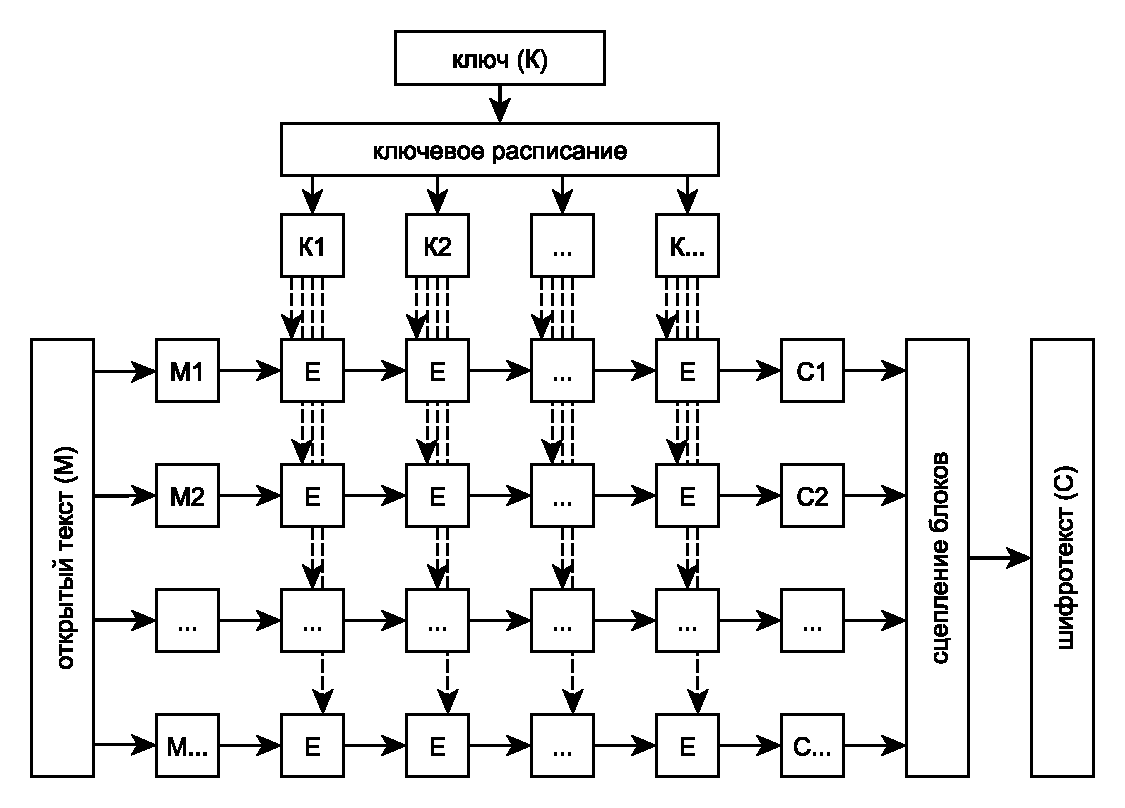
\includegraphics[width=1\textwidth]{pic/block-cipher}
  \caption{Общая структура блокового шифра. С помощью функции ключевого расписания из ключа $K$ получается набор раундовых ключей $K1, K2, \dots$. Открытый текст $M$ разбивается на блоки $M1, M2, \dots$, каждый из которых проходит несколько раундов шифрования, используя соответствующие раундовые ключи. Результаты последних раундов шифрования каждого из блоков объединяются в шифротекст $C$ с помощью одного из режима сцепления блоков}
  \label{fig:block-cipher}
\end{figure}

Все современные блоковые шифры являются \textit{раундовыми}. То есть блок текста проходит через несколько одинаковых (или похожих) преобразований, называемых \textit{раундами шифрования}. У~функции шифрования также может существовать начальный и завершающий раунды, отличающиеся от остальных (обычно -- отсутствием некоторых преобразований, которые не имеют смысла для <<крайних>> раундов).

Аргументами каждого раунда является результат предыдущего раунда (для самого первого -- часть открытого текста) и \textit{раундовый ключ}\index{ключ!раундовый}. Раундовые ключи получаются из оригинального ключа шифрования с помощью процедуры, получившей название расписание ключей\index{расписание ключей} (или же ключевое расписание\index{ключевое расписание}, англ. \textit{key schedule}). Функция ключевого расписания является важной частью блокового шифра. На потенциальной слабости этой функции основаны такие криптографические атаки, как атака на основе связанных ключей\index{атака!на связанных ключах} и атака скольжения\index{атака!скольжения}.

После прохождения всех раундов шифрования блоки $C1, C2, \dots$ объединяются в шифротекст $C$ с помощью одного из режимов сцепления блоков (см. раздел~\ref{chapter-block-chaining}). Простейшим примером режима сцепления блоков является режим электронной кодовой книги\index{режим!электронной кодовой книги}, когда блоки $C1, C2, \dots$ просто конкатенируются в шифротекст $C$ без дополнительной обработки.

К числовым характеристикам блокового шифра относят:
\begin{itemize}
	\item размер входного и выходного блока;
	\item размер ключа шифрования;
	\item количество раундов.
\end{itemize}

Также надёжные блоковые шифры обладают <<лавинным эффектом>>\index{лавинный эффект} (англ. \textit{avalanche effect}): изменение одного бита в блоке открытого текста или ключа приводит к полному изменению соответствующего блока шифротекста.